% !TeX root = ../../../book.tex
\subsection{直线划分平面区域}

取一张白纸、一支笔和一把直尺。纸上有多少个区域?只有一个,对吧?在纸上画一条直线。现在有两个区域。再画一条与第一条直线相交的直线。现在有多少个区域?数一数,总共有四个。绘制第三条直线,与前两条相交但不过其交点(即共产生三个交点)。现在有多少个区域?能否不通过计数预测结果?若有 $4$ 条直线呢?$5$ 条呢?$100$ 条呢?如何解决并最终推广此问题?让我们正式定义问题:

考虑无限平面(二维表面)上 $n$ 条互不\emph{平行}且无三条线共\emph{交点}的直线,它们将平面分割为多少个不同区域?

当 $n$ 较小时(如 $n \leq 5$),可通过手绘示例引导直觉,进而推广至\emph{任意} $n$。(此策略与前述问题相似:观察小规模模式,提炼可推广特征,最终抽象至一般情形。)具体而言,需探究新增直线如何\emph{改变}区域数量。绘制新直线时会发生什么?能否量化其创造的区域数?建议先自行思考本题,若得结论可与下文步骤对照。

让我们从 $n = 2$ 开始。已知单条直线将平面分割为 $2$ 个区域;添加第二条直线后如何变化?由绘图可知存在 $4$ 个区域:

\begin{center}
    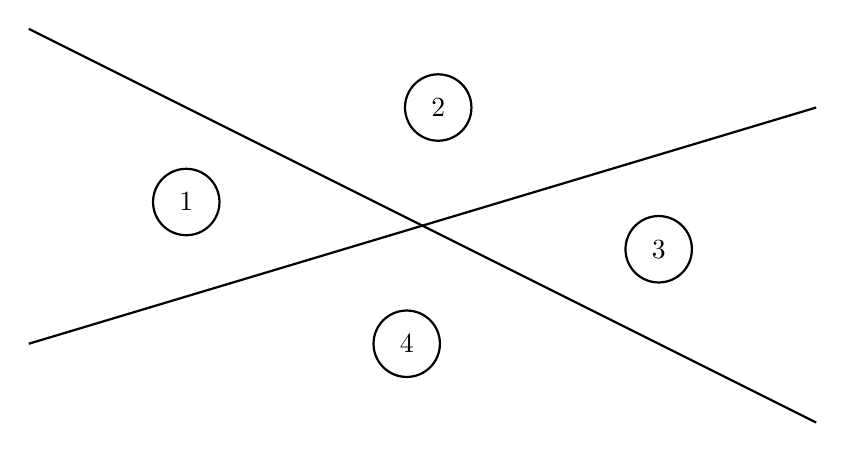
\begin{tikzpicture}[thick]
        \draw (-5,2.5) -- (5,-2.5);
        \draw (-5,-1.5) -- (5,1.5);
        \node[draw,circle,minimum size=24pt,inner sep=0,anchor=center] at (-0.2,-1.5) {$4$};
        \node[draw,circle,minimum size=24pt,inner sep=0,anchor=center] at (3,-0.3) {$3$};
        \node[draw,circle,minimum size=24pt,inner sep=0,anchor=center] at (-3,0.3) {$1$};
        \node[draw,circle,minimum size=24pt,inner sep=0,anchor=center] at (0.2,1.5) {$2$};
    \end{tikzpicture}
\end{center}

然而,这只是两条直线相交的\emph{特例}。如何证明\emph{任意}两条非平行直线\emph{总能}得到四个区域?也就是说,我们能否以某种方式结合直线数量 $n = 2$ 这一事实来描述这是\text{如何}发生的?思考一下!

下面是我们的方法。请注意,当我们添加第二条直线时,每个已经存在的区域都会被分成两部分,并且\emph{无论你如何绘制直线},只要确保两条直线不平行,结果都是这样。也就是说,如果我们用一条直线将平面分成两个区域,

\begin{center}
    \begin{tikzpicture}[thick]
        \draw (-5,2.5) -- (5,-2.5);
        \node[draw,circle,minimum size=24pt,inner sep=0,anchor=center] at (-3,0.3) {$1$};
        \node[draw,circle,minimum size=24pt,inner sep=0,anchor=center] at (0.2,1.5) {$2$};
    \end{tikzpicture}
\end{center}

然后添加一条新的直线会将每个现有区域分成两部分。这会向整个平面添加两个新的区域,总共四个区域:

\begin{center}
    \begin{tikzpicture}[thick]
        \draw (-5,2.5) -- (5,-2.5);
        \draw [color=red] (-5,-1.5) -- (0,0)  node[midway,below,sloped]{分割区域 1}
        -- (5,1.5) node[midway,above,sloped]{分割区域 2} ;
        \node[draw,circle,minimum size=24pt,inner sep=0,anchor=center,color=red] at (-0.2,-1.5) {$4$};
        \node[draw,circle,minimum size=24pt,inner sep=0,anchor=center,color=red] at (3,-0.3) {$3$};
        \node[draw,circle,minimum size=24pt,inner sep=0,anchor=center] at (-3,0.3) {$1$};
        \node[draw,circle,minimum size=24pt,inner sep=0,anchor=center] at (0.2,1.5) {$2$};
    \end{tikzpicture}
\end{center}

当 $n = 3$ 时呢?在这种情况下,我们需要考虑向具有两条直线和四个区域的图形中添加第三条直线。我们想要提出一个不依赖于线的特定排列的论证,因此我们最终唯一能用的事实是线之间互不平行,且任何交点仅位于两条线(而不是三条或更多)上。不过,就目前而言,查看特定的直线排列会有所启发,以便我们讨论相同的图形;我们可以利用对这个特定图形的观察来指导我们的一般论证。让我们从下方具有两条直线的图开始,向其中添加第三条直线,让第三条直线的交点都在初始交点``附近''或在图的范围内,这样我们就缩放图形了:

\begin{center}
    \begin{tikzpicture}[thick]
        \draw (-5,2.5) -- (5,-2.5);
        \draw (-5,-1.5) -- (5,1.5);
        \draw [color=red] (-5,1) -- (-1.8085,0.9043) node[midway,below,sloped]{\small 分割区域 1} 
        -- (2.5758,0.7727) node[midway,above,sloped]{\small 分割区域 2}
        -- (5,0.7) node[midway,below,sloped]{\small 分割区域 3};
        \node[draw,circle,minimum size=16pt,inner sep=0,anchor=center] at (-0.2,-1.5) {$4$};
        \node[draw,circle,minimum size=16pt,inner sep=0,anchor=center] at (3,-0.3) {$3$};
        \node[draw,circle,minimum size=16pt,inner sep=0,anchor=center] at (-3,-0.3) {$1$};
        \node[draw,circle,minimum size=16pt,inner sep=0,anchor=center] at (0.2,2) {$2$};
        \node[draw,circle,minimum size=16pt,inner sep=0,anchor=center,color=red] at (-4,1.45) {$5$};
        \node[draw,circle,minimum size=16pt,inner sep=0,anchor=center,color=red] at (0.1,0.45) {$6$};
        \node[draw,circle,minimum size=16pt,inner sep=0,anchor=center,color=red] at (4.61,1.05) {$7$};
    \end{tikzpicture}
\end{center}

很明显此时共有 $7$ 个区域。将第三条直线标绘为不同颜色,以便我们可以识别``新''区域出现的位置:一个区域(下方区域,区域 $4$)保持不变,但其他三个区域被一分为二,每次分割使区域计数加 $1$。如果我们以不同的方式绘制这条直线会怎样?

\begin{center}
    \begin{tikzpicture}[thick]
        \draw (-5,2.5) -- (5,-2.5);
        \draw (-5,-1.5) -- (5,1.5);
        \draw [color=red] (0,2.5) -- (-0.8333,0.4167) node[midway,right,sloped,rotate=-90]{\small 分割区域 2} 
        -- (-1.1364,-0.341) node[midway,left,sloped,rotate=-90]{\small 分割区域 1}
        -- (-2,-2.5) node[midway,right,sloped,rotate=-90]{\small 分割区域 4}; 
        \node[draw,circle,minimum size=16pt,inner sep=0,anchor=center] at (-0.2,-1) {$4$};
        \node[draw,circle,minimum size=16pt,inner sep=0,anchor=center] at (3,-0.3) {$3$};
        \node[draw,circle,minimum size=16pt,inner sep=0,anchor=center] at (-3,-0.3) {$1$};
        \node[draw,circle,minimum size=16pt,inner sep=0,anchor=center] at (1,2) {$2$};
        \node[draw,circle,minimum size=12pt,inner sep=0,anchor=center,color=red] at (-0.7,0.05) {$5$};
        \node[draw,circle,minimum size=16pt,inner sep=0,anchor=center,color=red] at (-1.5,1.8) {$6$};
        \node[draw,circle,minimum size=16pt,inner sep=0,anchor=center,color=red] at (-2.5,-1.4) {$7$};
    \end{tikzpicture}
\end{center}

类似的情况再次出现:其中一个区域保持不变,其余三个区域一分为二。(为何无其他区域?此问题值得深入思考。)尝试三条线的其他排列方式,并验证这种情况总会发生;此外,思考一下\emph{为什么}会出现这种情况,以及我们\emph{如何}解释这种情况一定会发生。不过,在给出一般性解释之前,我们再来看一下 $n=4$ 的情形。

当 $n = 4$ 时,我们从 $3$ 条直线和 $7$ 个区域的平面开始,添加第四条直线,该直线不与任何现有直线平行,并且不穿过任何现有交点。同样,我们想要提出一个与直线的特定排列无关的论证,但是查看下面的具体图形将有助于引导思路:

\begin{center}
    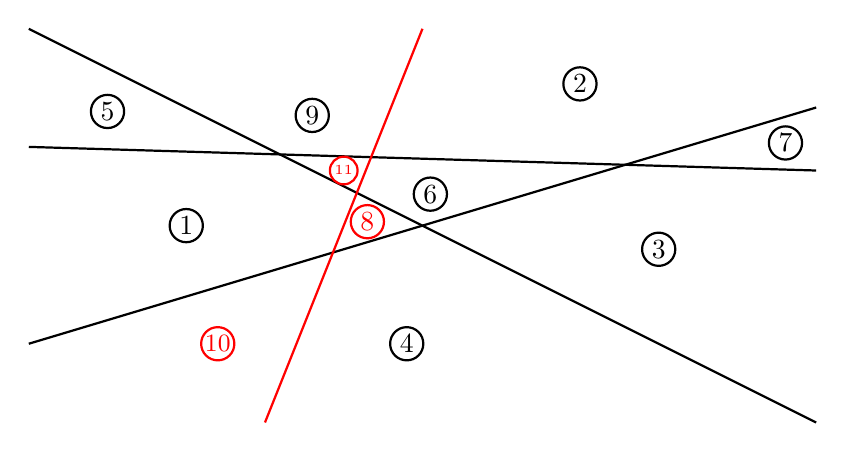
\begin{tikzpicture}[thick]
        \draw (-5,2.5) -- (5,-2.5);
        \draw (-5,-1.5) -- (5,1.5);
        \draw  (-5,1) -- (5,0.7);
        \draw [color=red] (0,2.5) -- (-2,-2.5);
        \node[draw,circle,minimum size=12pt,inner sep=0,anchor=center] at (-0.2,-1.5) {$4$};
        \node[draw,circle,minimum size=12pt,inner sep=0,anchor=center] at (3,-0.3) {$3$};
        \node[draw,circle,minimum size=12pt,inner sep=0,anchor=center] at (-3,0) {$1$};
        \node[draw,circle,minimum size=12pt,inner sep=0,anchor=center] at (2,1.8) {$2$};
        \node[draw,circle,minimum size=12pt,inner sep=0,anchor=center] at (-4,1.45) {$5$};
        \node[draw,circle,minimum size=12pt,inner sep=0,anchor=center] at (-1.4,1.4) {$9$};
        \node[draw,circle,minimum size=10pt,inner sep=0,anchor=center,color=red] at (-1,0.7) {\tiny $11$};
        \node[draw,circle,minimum size=12pt,inner sep=0,anchor=center] at (4.61,1.05) {$7$};
        \node[draw,circle,minimum size=12pt,inner sep=0,anchor=center,color=red] at (-0.7,0.05) {$8$};
        \node[draw,circle,minimum size=12pt,inner sep=0,anchor=center] at (0.1,0.4) {$6$};
        \node[draw,circle,minimum size=12pt,inner sep=0,anchor=center,color=red] at (-2.6,-1.5) {\small $10$};
    \end{tikzpicture}
\end{center}

请注意,三个原始区域保持不变(区域 $3$、区域 $5$ 和区域 $7$),而其他四个区域被一分为二。你注意到其中的规律了吗?对于每个已检验的 $n$,添加第 $n$ 条线会使 $n-1$ 个区域保持不变,其余区域则被一分为二。现在,让我们解释这一现象的原因。回忆一下,当绘制 $n$ 条直线时,我们的目标是确定区域的总数。为此,我们赋予该值一个名称以便引用:设 $R(n)$ 表示在平面上绘制 $n$ 条直线所创建的区域数,其中任意两条直线均不平行,且任意三条直线不共点。在上述示例中,我们考察了较小的 $n$ 值,并研究了添加新直线时的变化规律;也就是说,我们可以通过已知的 $R(n - 1)$ 推导 $R(n)$ 的值。现在,让我们将观察结果推广到适用于\emph{任意} $n$ 的情形。

假设已知 $R(n)$(为何可行?对于特定 $n$,我们是否确切知道 $R(n)$ 的值?它是什么?如何得知?)。考虑平面上满足题目条件的\emph{任意} $n$ 条直线图,这些直线将平面划分为 $R(n)$ 个区域。现在,添加第 $(n + 1)$ 条直线时会发生什么?关于这条直线如何改变图形,我们能确定哪些信息?关键约束如下:

\begin{enumerate}[label=(\alph*)]
    \item 新直线与现有的 $n$ 条直线均不平行;
    \item 新直线不经过任何现有交点。
\end{enumerate}

条件 (a) 表明新直线必与\emph{所有} $n$ 条已有直线相交(平行线无交点,非平行线必相交)。因此,新直线将产生 $n$ 个新交点。这些交点会与已有交点重合吗?不会!这正是条件 (b) 的作用。综上,只要满足题目要求,新直线上\emph{必定}存在 $n$ 个``特殊''点——即它与已有直线的交点。

接下来,我们利用这些特殊点识别新增区域。回顾之前的案例:标记新交点,并探究它们与新区域的关联。建议用圆点标记交点,并用 $\textbf{×}$ 标识新区域以增强可视性。下图展示了 $n = 4$ 的示例。你发现了什么?能否通过这些点推断添加第 $n$ 条直线后新增的区域数?思考一下,然后继续阅读。

\begin{center}
    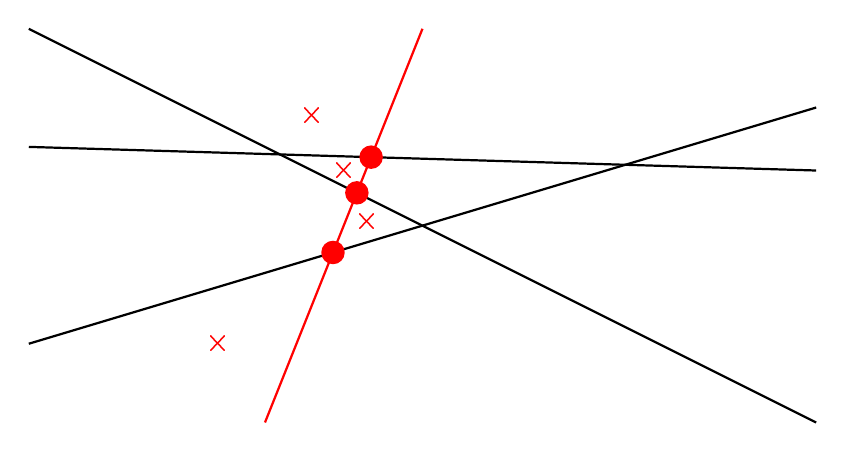
\begin{tikzpicture}[thick]
        \draw (-5,2.5) -- (5,-2.5);
        \draw (-5,-1.5) -- (5,1.5);
        \draw  (-5,1) -- (5,0.7);
        \draw [color=red] (0,2.5) -- (-2,-2.5);
        \node[minimum size=14pt,anchor=center,color=red,very thick] at (-1.4,1.4) {$\textbf{×}$};
        \node[minimum size=14pt,anchor=center,color=red,very thick] at (-1,0.7) {$\textbf{×}$};
        \node[minimum size=14pt,anchor=center,color=red,very thick] at (-0.7,0.05) {$\textbf{×}$};
        \node[minimum size=14pt,anchor=center,color=red,very thick] at (-2.6,-1.5) {$\textbf{×}$};
        \node[fill,circle,inner sep=3pt,color=red] at (-0.6522,0.8696) {};
        \node[fill,circle,inner sep=3pt,color=red] at (-0.8333,0.4167) {};
        \node[fill,circle,inner sep=3pt,color=red] at (-1.1364,-0.341) {};
    \end{tikzpicture}
\end{center}

没错!任意两个相邻新交点之间,都有一条\emph{线段}恰好将一个区域一分为二!接下来只需确定此类线段的数量即可。由于每条线段仅分割\emph{一个}已有区域,其数量即等于新增区域数。已知第 $(n + 1)$ 条直线产生 $n$ 个新交点。这些点在直线上如何排列?任意两个``连续'交点形成一条有限线段,而端点则延伸为无限射线(经端点无限延伸)。总计多少条线段?恰好 $n + 1$ 条(参考 $n = 3$ 的示意图:$3$ 个交点对应 $4$ 条线段,含两条无限射线)。因此,$n + 1$ 条线段分割出 $n + 1$ 个新区域,即:
\[R(n + 1) = R(n) + n + 1\]
出色的发现!通过分析示例和几何论证,我们成功揭示了递归关系:$R(n+1)$ 的值依赖于 $R(n)$。虽未完全解决问题,但已接近目标。接下来只需迭代展开 $R(n)$ 的表达式,直至已知的 $R(1) = 2$。过程如下:

\begin{center}
    \begin{tabular}{rcccccccccc}
        $R(n+1)$ & $=$ &          & &            &     &            &     & $\cancel{R(n-1)}$ & $+$ & $n+1$\\
                 & $=$ &          & &                   &     & $\cancel{R(n-1)}$ & $+$ & $n$ & $+$ & $n+1$\\
                 & $=$ &          & & $\cancel{R(n-2)}$ & $+$ & $(n-1)$           & $+$ & $n$ & $+$ & $n+1$\\
                 & $\vdots$ &     & &  &  &  &  &  &  & \\
                 & $=$ &          & & $\cancel{R(2)}+3$ & $+$ & $\dots$ & $+$ & $n$ & $+$ & $n+1$ \\
                 & $=$ & $R(1)+2$ & $+$ & $3$               & $+$ & $\dots$ & $+$ & $n$ & $+$ & $n+1$ \\
    \end{tabular}
\end{center}

由 $R(1) = 2$ 可得:
\[R(n + 1) = 2 + \left(2 + 3 + \dots + n + (n + 1)\right) = 2 + \left(\sum_{k=1}^{n+1}k\right)-1 = 1+\sum_{k=1}^{n+1}k\]
而这正是我们之前研究过的求和公式!(注意括号内求和缺首项 $k=1$,故需减去 $1$)。回忆 $\sum_{k=1}^{n} k = \frac{n(n+1)}{2}$,为了表示上面等式中的求和,我们只需将 $n$ 替换为 $n + 1$ 即可。因此,
\[R(n + 1) = 1+\frac{(n+1)(n+2)}{2}\]
最后,为得到 $R(n)$ 的显式表达式,将 $n+1$ 替换为 $n$(对 $n$ 的取值有什么要求?):
\[R(n + 1) = 1+\frac{n(n+1)}{2}\]
至此,我们获得了原问题的答案!此过程运用了\emph{归纳}技术:通过建立 $R(n + 1)$ 对 $R(n)$ 的依赖关系,反向迭代至\emph{已知}值 $R(1)$。

需要强调的是,本节推导旨在引导直觉而非提供\emph{严格证明}。省略号(``$\dots$'')并非严谨的数学归纳表述。此外,我们的方法是从 $n - 1$ 条直线出发\emph{逐步构建} $n$ 条直线的情形——这是否合理?为何能推广到 $n$ 条直线的\emph{任意}图?所有此类图是否均来自少一条线的子图?

接下来的两章将引入严格工具以形式化上述方法,并建立数学归纳的严谨框架。当前阶段,我们仅提供归纳法的启发式定义,并继续探索依赖归纳的有趣问题。重点在于练习识别归纳结构、运用其解决问题等技能,这对未来学习至关重要(暂无需深入数学细节!)。
